In this chapter I will provide general review of single cell transcriptomics and related challenges.

\section{Introduction to single cell transcriptomics}

Cells are the fundamental units of life, forming the basis of all living organisms.
One of the major goals of biology is to understand cellular systems and the processes occurring within cells.
Since the discovery of the DNA structure in 1953
and the development of the conceptual framework for genetic information transfer,
scientists have made significant efforts to sequence the genomes of various organisms.
This led to the development of the first sequencing methods, such as Sanger sequencing in 1975,
which laid the foundation for next-generation sequencing (NGS) technologies in use today,
including the widely used Illumina platform (\cite{Heather2016}).
Current sequencing methods allow us to obtain the complete genetic sequence of any organism.
However, the genome alone cannot explain the full diversity of cells in multicellular organisms,
as all cells share the same genome but exhibit significant variation in shape, size, and function.

RNA sequencing (RNAseq), on the other hand, enables the measurement of gene expression within cells,
providing valuable insights into cellular processes.
RNAseq methods largely follow DNA sequencing protocols,
with the addition of a step where complementary DNA (cDNA) is synthesized from RNA (\cite{Heumos2023}).
The first RNAseq methods were developed for bulk sequencing, where RNA from entire cell populations is sequenced,
providing an average gene expression profile across the population.
Although bulk RNAseq has provided valuable insights into the dynamics of cellular processes
(such as changes in disease states in response to therapeutics, detection of gene isoforms, gene fusions,
and various other properties of target cells (\cite{Heumos2023})),
this approach masks non-dominant processes and cell-to-cell variability through averaging.
This limitation was addressed by the introduction of single-cell RNA sequencing (scRNAseq) methods,
which allow for the generation of transcriptomic profiles from individual cells,
providing high-resolution insights into cellular systems.

Current scRNAseq methods enable the generation of transcriptomic profiles from thousands of cells
at unprecedented resolution in a single experiment.
These data can be used for constructing cellular atlases (\cite{Rozenblatt2017}),
understanding disease mechanisms (\cite{Zhang2024}),
exploring cell differentiation and developmental processes (\cite{Skinner2024}), among many other applications.

\section{Key methods and technologies in scRNAseq}

\subsection{Key methods}

All scRNAseq protocols share these main three steps:
isolation of single cells, library preparation and sequencing (\cite{Andrews2018}).

The first step is mainly done in two ways:
either by placing cells in separate droplets (microfluidics approach),
or by separating cells into different wells (plate-based approach).

The next generation sequencing (NGS) usually requires nanograms or more of DNA,
and the RNA content in single cells is far from this amount (\cite{Wu2017}).
Consequently, before sequencing, reverse transcription (RT) and amplification is needed.

Finally, the prepared library is sequenced using NGS methods.
The most popular is ........

\subsection{Current scRNAseq Platforms}

As mentioned before, scRNAseq methods mainly can be grouped in two groups: droplet-based and plate-based.

Droplet-based methods (e.g. inDrops (\cite{Klein2015}), Drop-seq (\cite{Macosko2015}),
Chromium by 10X Genomics (\cite{Zheng2017}))
separate cells by placing them into different droplets, which contain hidrogel primers and lysis mix.
Primers usually share a common structure, including barcode sequenes, unique molecular identifiers (UMIs),
PCR handlers and poly-T sequences (\cite{Zhang2019}).
Cell barcodes are sequences used for determining the cell from which a particular read was sequenced
(during sequencing, the content from all droplets is mixed and sequenced at once).
UMIs are used to quantify real amount of RNA in cells
(after amplification, more than one copy of each captured RNA is present).
PCR handlers are used for the amplification, while poly-T sequences are used for capturing RNAs.
An example of primer design can be seen in figure \ref{fig:primer}).
Once cells are in the droplets, cell lysis takes place, RNAs escape the cells and are captured by the primers.
Depending on method,
reverse transcription either takes place directly in the droplets (inDrops, 10X) or after demulsification (Drop-seq).
The next steps usually include RNA fragmentation and PCR amplification, followed by NGS.

Droplet-based methods are high-throughput
(current microfluidic devices are able to generate thousands of above described droplets per second (\cite{Prakadan2017})),
cost-effective, but have low detection rates compared to other methods and
captures only 3' (or 5') ends of transcripts (\cite{Heumos2023}).
Capturing only 3' ends of transcripts might be not a problem when trying to identify cell populations,
however, it masks such processes as splicing variants, thus should be considered carefully when planning experiments.

Plate-based methods (e.g. CEL-Seq2 (\cite{Hashimshony2016}), Smart-seq2 (\cite{Picelli2013}))
separate cells by placing them into different microwells on a plate.
Before this, cells can be sorted using, for example, fluorescent-activated cell sorting (FACS) (\cite{Heumos2023}).
Similarly to droplets, microwells contain lysis buffers and RT mix,
followed by amplification and NGS (\cite{Hashimshony2016}).
Barcodes can be integrated into reverse transcription step similarly as in droplet case.

Overall, plate-based methods have lower throughput, might be more costly and labor-intensive,
but offers recovery of many genes per cell, allows prior sorting and
(for some protocols) it is possible to sequence full transcripts (\cite{Heumos2023}).

In the next sections, we will focus on the droplet-based approaches,
as all the data used in this thesis is generated by droplet-based methods.

\begin{figure}
  \centering
  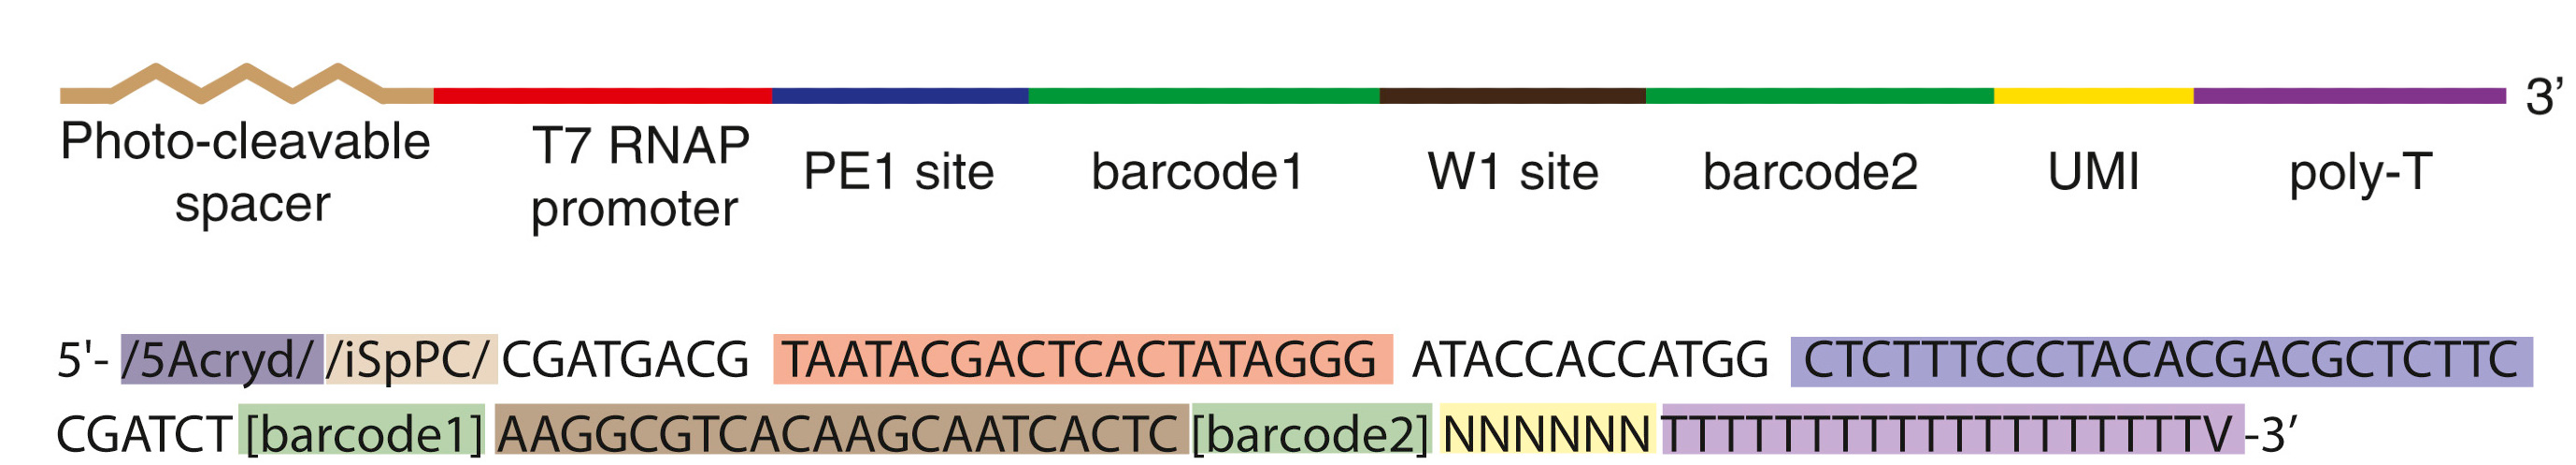
\includegraphics[width=\linewidth]{images/primer.png}
  \caption{Example of barcode (inDrops). Image taken from (\cite{Klein2015}).}
  \label{fig:primer}
\end{figure}

\section{Data quality and challenges in scRNAseq data}

The quality of scRNAseq data

\subsection{Noise}

dropout, sparsity, batch effects, doublets, ambient RNA,

The noise present in the scRNAseq data can be either biological or technical.

\subsection{Dimentionality}

\section{Computational tools and analytical approaches}

\subsection{Raw data processing}

The output of the typical scRNAseq experiment is FASTQ files, containing recorded sequences,
as well as (depending on method) barcode and UMI sequences, and quality scores.
The subsequent processing steps include quality control of FASTQ file (based on quality scores),
filtering dublicate reads (using UMIs), mapping reads to the genome sequence, assigning the reads to the genes,
and finally, counting gene expression per cell (barcode) (\cite{Heumos2023}) (see figure \ref{fig:rawData}).
Usually, all these steps are performed with a single piece of dedicated software,
such as STARsolo (\cite{Kaminow2021}), CellRanger (\cite{Zheng2017}) or others.
It should be noted, that there are variations in the pipeline described above,
depending on many experiment-related (e.g., whether the genome sequence or transcriptone of the study organism is known),
or method-related (e.g., whether UMIs are used in the protocol) factors.
The typical result of such processing is cell-gene matrix (i.e., a matrix where rows represent cells,
columns represent genes, and each entry indicates the number of captured RNAs for a given gene in a specific cell).

\begin{figure}
  \centering
  
\includegraphics[width=\linewidth]{images/rawdata.png}
  \caption{Pipeline of processing raw data.}
  \label{fig:rawData}
\end{figure}

\subsection{Preprocessing of count matrices}

Preprocessing of count matrices usually involves these steps:
quality control, normalization and feature selection.

The quality of indidual cells can be evaluated based on several factors, such as mitochondrial gene content
(apoptotic cells tend to have a higher proportion of mitochondrial genes (\cite{Heumos2023})) or
total number of captured genes (very low numbers can be produced by empty droplets).
In some cases, two cells can end up in one droplet,
resulting in count matrix row corresponding to genes from  both cells.
Such matrix entries (doublets) can be filtered by using specialized software
such Scrublet (\cite{Wolock2019}) or scDblFinder (\cite{Germain2022}).
Another source of noise in scRNAseq data is ambient RNA,
which consists of RNA that escapes individual droplets and spreads into the medium or other droplets,
leading to background noise.
Even though the amount of such RNA is not high (in good quality datasets it can be around 2\% (\cite{Young2020})),
removing these RNAs from the count matrix can improve data quality.
This can be achieved by identifying the background noise profile from empty droplets and
adjusting the count matrix accordingly.
There are dedicated softwares,
such as SoupX (\cite{Young2020}), decontX (\cite{Yang2020}), CellBender (\cite{Fleming2023}) and others.

The next step in preprocessing pipeline is normalization.
The goal of normalization is to transform the data so that the variation in gene expression levels is comparable,
making subsequent analysis more efficient (\cite{Ahlmann2023}).
Normalization can also help eliminate biases,
such as differences in sequencing depth when combining data from multiple samples (\cite{Lingen2024}).
There are numerous normalization methods, based on different approaches
(e.g., delta-method-based, residual-based, latent gene expression-based, count-based (\cite{Ahlmann2023})).
Thus, selecting a normalization method should be done carefully, depending on the experimental design.
General recommendations for normalization suggest comparing several methods,
and if the results are similar, opting for the simpler method (\cite{Lingen2024}).
Sophisticated methods do not necessarily show better results, and a recent benchmarking study by \textcite{Ahlmann2023}
has shown that simpler method (particularly the logarithm normalization,
where each element $y$ of count matrix is transformed by formula $y_{trnasformed} = log(y+1)$)
performs as well or better than more advanced methods.

Once the data is normalized and cleaned, one can filter out non-informative genes.
Initially, count matrices contain all the genes that are present in the transcriptome.
However, not all of them are expressed in the sequenced data, or are expressed in negligable numbers (\cite{Heumos2023}).
Therefore, it is common practice to filter such genes (e.g., genes that are expressed in less than three cells).
Moreover, some genes might be expressed in all the cells more or less evenly (housekeeping genes),
which do not provide useful information that could be usefull in, for instance, grouping cells or determining cell types.
Therefore, in many applications, it is beneficial to leave only those genes, that are highly variable between cells.
In such way, the dimensionality of the count matrix is greatly reduced without loosing significant information.
Additionally, genes that are outside the scope of the specific study can also be filtered out.

\subsection{Dimensionality reduction}

Even after filtering and selecting only highly variable genes, several thousand genes usually remain.
It is not feasible to visualize (and hard to interpret in general) data of such high dimentionality, therefore,
dimensionality reduction is essential step of subsequent analysis.
The idea of dimentionality reduction is simple:
to reduce the dimentions of the data loosing as little information as possible.
There are number dimensionality reduction methods based on different mathematical concepts,
but the most widely used today include
t-SNE (\cite{Hinton2002}), UMAP (\cite{McInnes2018}) and principal component analysis (PCA).
Although the use of these algorithms are supported by some benchmarking studies
(in the study of \textcite{Xiang2021}, t-SNE was showed best performance, while UMAP showed the highest stability),
other benchmarking studies report different findings.
The study of \textcite{Koch2021} suggested that such overlooked methods as
latent Dirichlet alloacation (LDA) and PHATE show best performance.
Meanwhile \textcite{Sun2019} provided guidelines for choosing dimensionality reduction method
depending on downstream analysis tasks, and in their results UMAP and tSNE were not on the top choices.
Thus, while UMAP and t-SNE remain the most popular methods in the field,
it is worth considering alternative methods as well.

\subsection{Clustering and other analyses}

One of the most popular tasks of scRNAseq data analysis is to identify and classify cell populations (\cite{Andrews2018}).
This task requires to assign cells to different groups (clusters),
such that cells in the same clusters are similar and distinct from cells in other clusters.
There is a great variety of clustering algorithms available,
including k-means, hierarchical and consensus clustering (\cite{Peng2020}).
Benchmarking studies suggest that "no individual scRNA-seq clustering algorithm can capture true clusters and achieve
optimal performance in all situations" (\cite{Peng2020}).

Clustering is usually followed by cell typing (i.e., assigning cell type to the identified clusters),
which is done by finding cell type specific markers
or using automatic (machine learning) tools such as CellTypist (\cite{Dom2022}).
The subsequent steps in the analysis depend on the focus of the particular study and can include
analysis of the dynamics of cellular systems (RNA velocity, pseudotime),
inferring gene regulatory networks (GRNs), and more.

\section{Enhancing scRNAseq data}

Given the challenges associated with scRNAseq data, there have been attempts to improve the quality of such data.
In this section, I will provide an overview of two methods: data imputation and enhancing the transcriptomic reference.

\subsection{Data imputation}

One of the challenges present in scRNAseq data is the large number of dropout values.
Dropout values refer to instances where gene expression is present in a cell but is missed in the scRNAseq data.
This problem can mask important relationships between genes and complicate downstream analysis (\cite{Wang2022}).
To impute dropout values, many tools have been suggested.
These methods can be divided into four categories:
model-based methods (bayNorm (\cite{Tang2019}), BISCUIT (\cite{Azizi2017}), SAVER (\cite{Huang2018}) etc.),
low-ranked matrix-based (ALRA (\cite{Linderman2022}), ENHANCE (\cite{Wagner2019}), scRMD (\cite{Chen2020}) etc.),
data smoothing methods (e.g. KNN-smoothing (\cite{Wagner2017}), MAGIC (\cite{Dijk2018}) etc.) and
deep learning methods (e.g. DCA (\cite{Eraslan2019}), DeepImpute (\cite{Arisdakessian2019}) etc.) (\cite{Wang2022}).

The study by \textcite{Dai2022} has shown that imputation methods are advantageous for recovering gene expression,
and among these methods, deep learning-based ones,
such as DCA, DeepImpute, scIGANs (\cite{Xu2020}) show the best performance.
However, it was also shown that imputation methods can introduce false positives.
In the study by \textcite{Andrews2019}, it was shown that data smoothing methods (e.g. MAGIC, KNN-smoothing)
generate most false positives among the different types of methods,
but other methods can generate relatively large number of false positives as well, depending on the dataset.
Data imputation does not necessarily improve downstream analysis
(e.g, it was shown that imputation doesn't improve inference of gene regulatory networks (\cite{McCalla2023})),
therefore one should carefully choose whether to impute data and which method to use.

\subsection{Enhancing transcriptomic reference}

One of the problems that scRNAseq is facing is the complexity of the genome.
The "raw" human transcriptomic reference (a file containing information about genes)
contains over 60000 genes (\cite{Frankish2022}).
Not all of these genes are expected to be captured by scRNAseq data
Thus, a simple approach to improving the transcriptomic reference is to filter out the genes
that are not expected to appear in scRNAseq data.
In this way, events where two genes overlap in the genome, but one is not expected to appear in the scRNAseq data,
are resolved, allowing alignment tools to more easily assign reads from these regions to the correct genes.
This approach is used in publicly available 10X transcriptomic references (\cite{Zheng2017}).
Even though it improves mapping performance, it does not address all the issues with the transcriptomc reference.

\textcite{Pool2023} has suggested three steps to enhance transcriptomic reference:
including reads mapped to intronic sequence to the analysis, extending 3' ends of some genes and
resolving overlaps between certain genes.
The first suggestion is not new in the field of scRNAseq.
There are concepts such as RNA velocity based on spliced an unspiced RNA ratio (\cite{Manno2018}),
showing that such including intronic reads in the analysis can provide valuable information.
Moreover, most mapping tools (e.g. STARsolo, CellRanger) contains options
to use either only exonic parts or full genes for read alignment.
The second suggestion is based on the observation,
that scRNAseq data often contains peaks of reads just after the 3' end of genes. 
While the exact biological reasons for this are unclear,
it makes sense to associate these reads with the genes they are closest to. 
The third suggestion focuses on resolving overlaps between genes.
Reads from such overlapping regions are often unassigned to any gene,
but in some cases, it is more likely that they originate from one gene rather than another.
Overlapping gene resolution aims to address this by deleting or shortening some genes in the transcriptomic reference.

Although \textcite{Pool2023} proposed the tool for such tasks, the tool is not without limitations:
some aspects of it are debatable (such as thresholds used), some seem unnecessarily
(e.g. handling exon and intron sequences when most alligning tools provide option for this),
and the process still requires a significant amount of manual work.
Thus, there remains a need for a more comprehensive tool for enhancing transcriptomic references,
which will be addressed in this thesis.

\section{Getting insights from scRNAseq data}

\subsection{Pseudotime and RNA velocity}

\subsection{Inferring gene regulatory networks}

\subsection{Integrative approaches}

\section{Current limitations and future perspectives}

